\section{Versuchsaufbau und Versuchsdurchführung}

\begin{flushleft}
    Zusehen ist der Versuchsaufbau in der Abbildung \ref{Abbildung5}. 
    Der Aufbau besteht aus einem Oszilloskop, einem Spannungsgenerator, einem Verstärker, einem Zählratenmesser, einer bzw. zwei $\beta$-Strahlungsquellen und einem Geiger-Müller-Zählrohr.
    Der Spannungsgenerator wird mit dem Geiger-Müller-Zählrohr verbunden, welches ebenso mit dem Zähler verbunden ist. 
    Über den Zählratenmesser wird das Signal verstärkt über den Verstärker und auf dem Oszilloskop projiziert.
    Das Geiger-Müller-Zählrohr befindet sich mit den $\beta$-Strahlenproben in einem Aluminiumkasten.
\end{flushleft}

\begin{figure}[H]
    \centering
    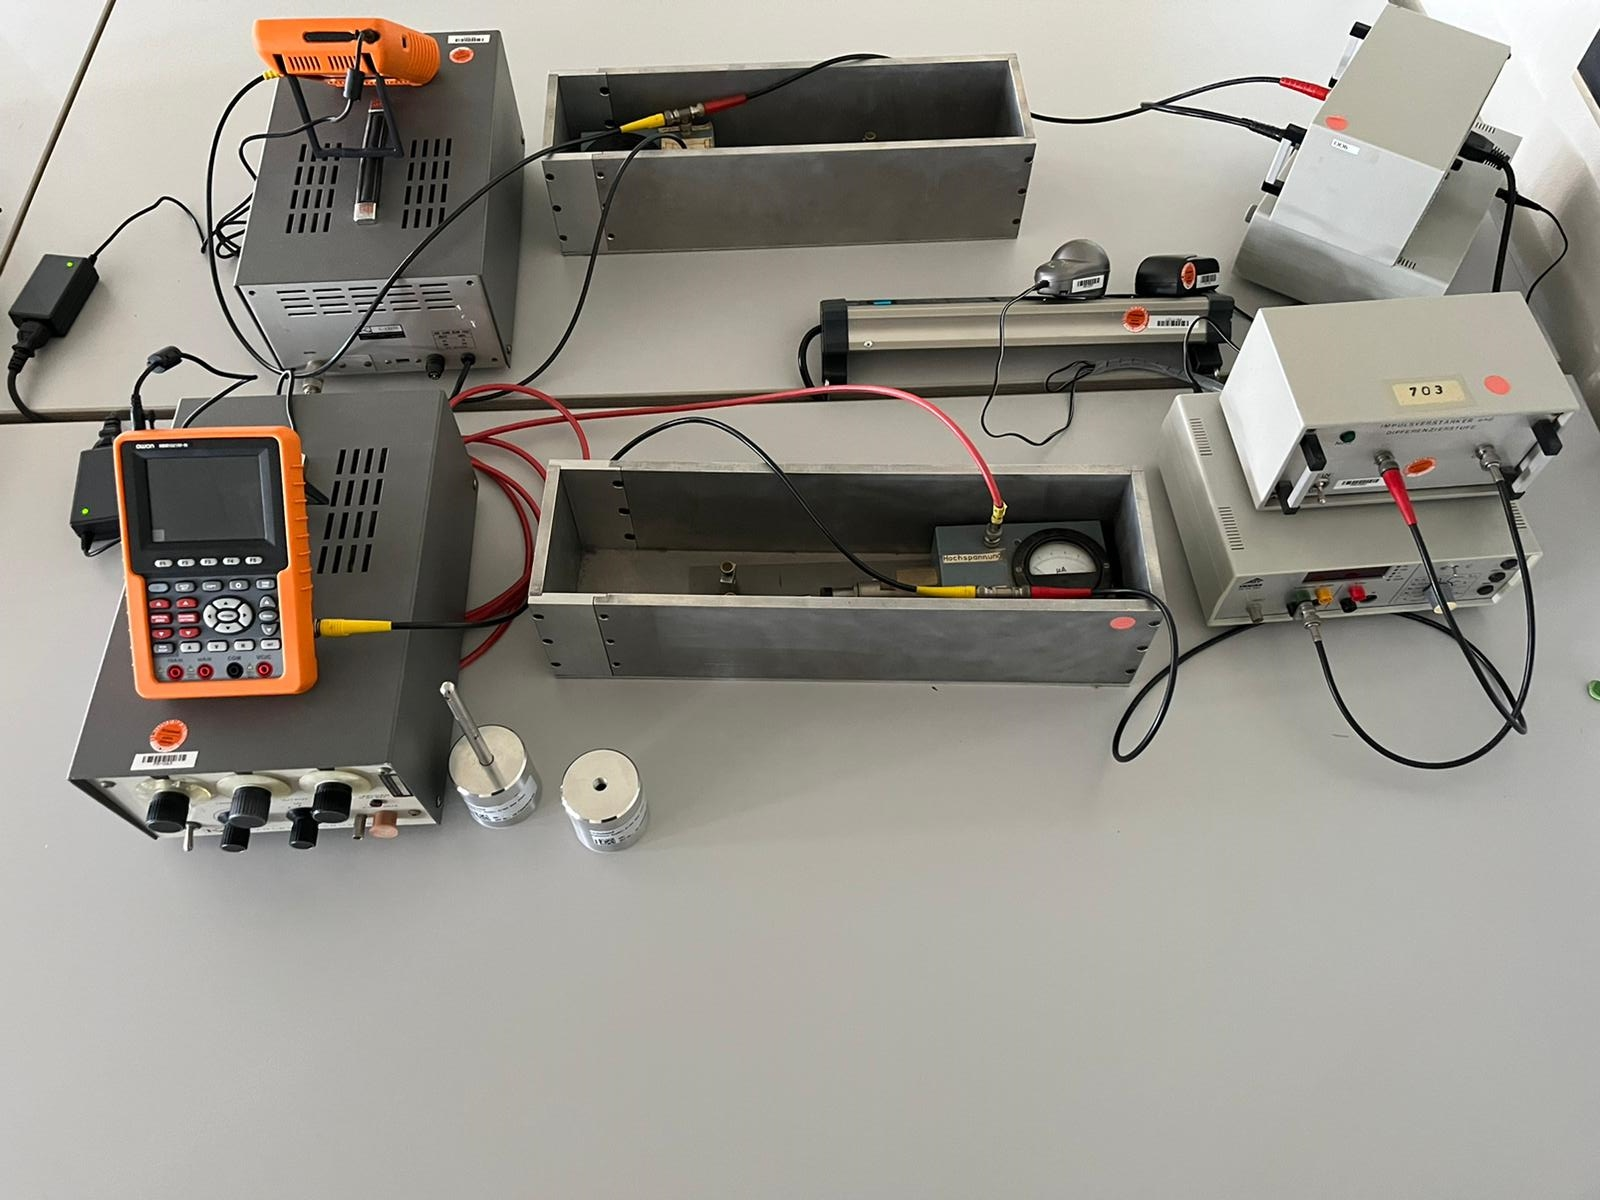
\includegraphics[height=80mm]{bilder/Ab5.jpeg}
    \caption{Die Abbildung zeigt den gesamten Versuchsaufbau.\label{Abbildung5} }
\end{figure}

\subsection{Bestimmung der Zählrate von \textbeta -Strahlung}

\begin{flushleft}
    Der Aufbau wird wie in Abbildung \ref{Abbildung5} aufgebaut. 
    Zuerst wird der Timer des Zählratenmessers auf $60\,\unit{\second}$ und die Spannung von auf $320\,\unit{\volt}$ gestellt.
    Danach wird die $\beta$-Strahlenproben in den Aluminiumkasten vor das Geiger-Müller-Zählrohr platziert. 
    Aufgenommen werden die Zählrate und der Strom, welcher auf dem Geiger-Müller-Zählrohr abzulesen ist, notiert.
    Dies wird für die Spannungen $320\,\unit{\volt} \leq x \leq 700\,\unit{\volt}$, in jeweils $10\,\unit{\volt}$ Schritten, wiederholt.
\end{flushleft}

\subsection{Bestimmung der Tot- und Erholungszeit mithilfe eines Oszilloskops}

\begin{flushleft}
    Der Aufbau wird nicht verändert.
    Als nächstes wird die Spannung auf $500\,\unit{\volt}$ gestellt und der Verlauf auf dem Oszilloskop wird fotografiert.
\end{flushleft}

\subsection{Bestimmung der Tot- und Erholungszeit durch Zwei-Quellen-Methode}

\begin{flushleft}
    Der Aufbau wird erneut nicht verändert.
    Diesmal wird der Timer des Zählratenmessers auf $120\,\unit{\second}$ und die Spannung von auf $500\,\unit{\volt}$ gestellt.
    Danach werden drei verschiedene Messungen durchgeführt.
    Zuerst wird die Messung für die erste Probe, isoliert, durchgeführt.
    Danach wird die Messung für die zweite Probe, ebenfalls isoliert, durchgeführt.
    Und als letztes werden beide Proben gleichzeitig in dem Kasten platziert und die Zählrate aufgenommen.
    Wichtig dabei zu beachten ist, dass die Zählrate der beiden isoliert aufgenommenen Proben zusammen addiert höher ist als die der gleichzeitig verwendeten Proben. 
\end{flushleft}